\section{Overview}
In this section, we introduce the data model, discuss the problem, and finally, present a brief overview of existing solutions as well as our approach.

\subsection{Data} We focus on heterogeneous Web data including relational data, XML, RDF and other types of data that can be modeled as graphs. Closely resembling the RDF data model, we employ a graph-structured data model where every dataset is conceived as a graph $G \in\mathbb{G}$ comprising a set of triples: 

\begin{definition}[Data Model] A dataset set is a graph $G$ formed by a set of triples of the form $(s, p, o)$ where $s \in U$ (called subject), $p \in U$ (predicate) and $o \in U \cup L$ (object). Here, $U$ denotes the set of Uniform Resource Identifiers (URIs) and $L$ the set of literals. Every literal $l \in L$ is a bag of tokens, $l = \{t_1,\ldots,t_i,\ldots,t_n\}$, drawn from the vocabulary $V$, i.e. $t_i \in V$.  
\end{definition} 

With respect to this model, \emph{instances} are resources that appear at the subject position of triples. An instance representation can be obtained from the data graph as follows:

\begin{definition}[Instance Representation] The instance representation $IR: U \times \mathbb{G} \rightarrow \mathbb{G}$ is a function, which given an instance $s \in U$ and a graph $G \in \mathbb{G}$, maps $s$ to a set of triples in which $s$ appears as the subject, i.e. $IR(s) = \{ (s, p, o) | (s, p, o) \in G, o \in L \}$. 
\end{definition} 

Thus, an instance is basically represented through a set of \emph{predicate-value} pairs, where values are bags of tokens. \todo{add a graph to provide example, also, provide one example for instance representation} 
We will use the terms instance and instance representation interchangeably from now on. Note that for the sake of presentation, only the outgoing edges $(s, p, o)$ of an instance $s$ are considered while incoming edges (triples where $s$ appears as the object) can also be added to the representation of $s$. 

\subsection{Problem - Computing Instance Matches and Instance Match Candidates} \emph{Instance matching} is about finding instances that refer to the same real-world object based on their representations extracted from the data. In this paper, we tackle the problem of \emph{instance matching across multiple datasets}: given instances of a \emph{source dataset} $G_s$, the problem is to find instances in other datasets, collectively referred to as the \emph{target dataset} $G_t$, which represents the same real world object. 

Compared to the single dataset setting, this problem entails additional challenges especially when the data is heterogeneous not only at the data but also schema level. In this regard, \emph{data-level heterogeneity} means that for the same property, instances referring to the same object may have different values, or different syntactical representations of the same value. \todo{For instance, the values "Michael Jackson" or "Jackson, Michael" can be both used as the value of the property name of an instance representing  Michael Jackson.} Schema-level heterogeneity arises when there is only little or no schema overlaps between the datasets. That is, instances referring to the same object may be represented by different predicates, or different representations of the same predicates. Finding different representations of the same predicate is part of a problem also known as schema matching. 

More precisely, instance matching can be formulated as the problem of finding a (weighted) combination of similarity function predicates, $\sum_i{w_i s_i(p_m,p_n)} > \alpha$, which can be used to decide if a given pair of instances match (when the similarity exceeds the threshold $\alpha$), or not. Every $s_i(p_m,p_n)$ is a similarity function, which given the values of the predicates $p_m$ and $p_n$, returns a similarity score. This problem entails the subproblems of finding the comparable predicates $p_m$ and $p_n$ (schema matching), choosing and weighting these predicate pairs, as well as determining the similarity function $s_i$ (e.g. Jaccard distance) and threshold $\alpha$.  

Often, instance matching is preceded by a blocking step, which aims to quickly select candidates matches (hence also referred to as the \emph{candidate selection} step). Instead of using a combination of similarity function predicates, candidate selection simply employs a (conjunction of) blocking key(s), i.e. $\bigwedge s_i(p_m,p_n)$, where $s_i$ is a binary function that returns whether the two values of $p_m$ and $p_n$ match or not. Here, the predicates $p_m$ and $p_n$ constitutes the pair of comparable blocking keys while their values are called \emph{blocking key values} (BKV). Usually, the similarity function is fixed to be exact value matching or value overlap. That is, two instances form candidates if their blocking key values are the same or overlap on some tokens. In this step, there is no need of tuning any threshold. However, quite often, candidate sets are refined in a intermediary matching step by a matcher based on on approximate string matching over the BKVs. 

Thus, candidate selection can be seen as sub-problem of instance matching, i.e. finding comparable predicate pairs and choosing the most selective as blocking key pairs. Fig. 1 depicts the whole instance matching process described here. This paper focus on the candidate selection part of the problem.

 \begin{figure} [ht]
 
\centering
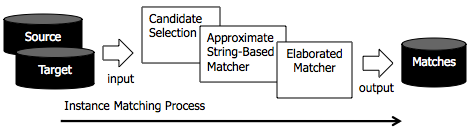
\includegraphics[scale=0.5]{p1.png}
\caption{Instance matching process overview.} 
\vspace{-2pt}
\label{fig:space}
\end{figure}

 

\subsection{Existing Solutions} Most of the approaches that tackle the candidate selection problem over heterogeneous data, where there are no overlaps between schemas, i.e. predicates in different datasets do not matches, uses an approximate string matching-based matcher to resolve the ambiguity(imprecision) on candidate sets that contains instances that share overlapping strings. One main class of solutions for this problem comprises supervised learning-based approaches, which uses training examples to learn the comparable predicates, the similarity functions and their thresholds. 

For instance,\cite{DBLP:conf/vldb/ChaudhuriCGK07} exploits the availability of positive and negative examples to search through this space and suggest an initial record matching query. Although they do not learn the comparable predicates, their algorithm find the combination of $s_i(p_m,p_n)$ and their respective threshold that produces the best candidate sets, i.e., those that include all positive matches and avoid the negative ones. As a limitation of this approach,  it requires positive and negative examples that are hard to obtain, specially in the heterogeneous settings; moreover, this approach can be problematic when applied over remote data endpoints.
 
Another class of solutions for this problem comprises unsupervised learning-based approaches, which without training examples, try to learn the comparable predicates, their mapping, the similarity functions and thresholds, by only inspecting the data and schema.

 
The problem of learning/finding comparable predicates in this setting is presented in \cite{DBLP:conf/semweb/SongH11}. To determined the comparable predicates, they compute the coverage and the discriminability of all predicates, by counting the frequency that each predicate occurs in the data; then predicates with high discriminating score that are above are threshold are considered as comparable predicates. When individual discriminabilities are below the threshold, predicates are combined together to become more discriminative. The threshold is manual defined, and in the worse case can lead to an exponential combination of keys. Beside of that, the mapping between those source and target predicates are manually defined (another limitation of their work). Then, after the comparable predicates are manually mapped, the instances are indexed by the value of those predicates and the candidate sets are formed by searching on this index for overlapping tokens. Because candidate selection are generally imprecise, a approximate string-based matcher is applied to prune the candidates that are above a threshold. In this step, both the similarity function and the threshold are manually defined. Finally, the candidates sets generated are delegated to an arbitrary more elaborated matcher that finds the exact matches. 

Another unsupervised solution is described in \cite{DBLP:conf/wsdm/PapadakisINF11}. They describe  a schema-agnostic approach to solve the sub-problem of candidate selection. In their approach, the learning of comparable predicate is unnecessary. They based on the idea that instances that refer to the same entity have at least one value in common, independently of the corresponding predicate names. Therefore, all instances that contain the same token in any predicate are placed in one candidate set (block, in their terminology). The approach is thus very robust against heterogeneity, noise, and loose schema binding. However, the candidate sets produced are highly redundant, because each instance is placed in multiple candidate sets. Consequently, a lot of processing is required to efficiently build precise candidate sets. Although, the authors states that in this setting the use of schema knowledge improves the precision but decreases considerably the coverage of the correct matches, we will show that the use of the predicates in the blocking keys can considerably improve the performance of both measures. 

\subsection{Our Solution}

To tackle the time issue described before we need to generated highly selective blocking scheme individually for each source instance, which can quickly produce optimal candidate sets. We use a specific approximate string matching based matcher during the process to generate positive and negative examples. Later, those examples are used in the process to refine the blocking schema. Because we need to query the remote data endpoint using those blocking schemes, we pose the candidate selection problem as an optimization problem, where the goal is to find the most selective conjunction of query clauses (blocking keys) that maximizes the correct matches in the candidate sets and minimizes the incorrect ones.

\begin{definition} [Template Query]  A template query Q is conjunction of $n$ tuples $(p, k)$, where $p$ is a predicate in $G_t$ and $k$ is a token, defined as $ \bigwedge_{i}^n (p_i, k_i)=\{t | (t,p_i,o) \in G_t  \land o \sim k_i  \}$. The similarity function $\sim$ is given. Without loss of generality we can also assume that can exist tuples where p are undefined, acting as a wild card. 
\end{definition} 
 
\begin{definition} [Candidate Set]  A candidate set of an instance s in $G_s$ is a instantiation of a template query Q where we have at least a tuple $(p,k)$ where $(s,x,k) \in IR(s)$
\end{definition} 

\textbf{Solution overview}. Aiming to approximate our solution to the optimal solution, we approach this problem in an iterative fashion, where at each iteration we use information from the previous iteration to refine and increase the selectivity of the query templates used on next iterations. Notice that as more selective a query is, as more efficient and effective it is, because, it selects less elements(and it takes less time); and it selects less incorrect matches.  

Without any knowledge of the source or target schemas, we start the process with queries templates that are less selective but easy to build. As the process moves on, information obtained from the candidate sets produced in previous iterations are used to refine the query templates for next iterations. Basically, this refining process adds two types of clauses in the query templates, aiming to make them more selective: attribute and class clauses. Attributes clauses are composed of highly selective target predicates with values similar to the values of at least one highly selective source predicate. The value of this source predicate is used as the object value of the attribute clause. To build attribute clauses we apply an extension of Algorithm 2 described in our previous work \cite{•} over the source instances and instances in the candidate sets already generated. Class clauses are predicate/value pairs that represent the class of interest of the target instances (e.g. rdfs:type=geo:country). To build class clauses, we apply a matcher over the already generated candidate sets obtaining positive and negative examples. Then, those positive and negatives examples are input to an algorithm that output the set of predicate/value pairs that select all positives and avoid the negatives examples; namely, the class of interest. Finally, those pairs are used to compose the class clauses. The matcher can be any approach that uses a more complex similarity measure to select the correct matches (positive examples) among the possible candidates. In this work, we assume that the source instances belong to a specific class of interest (e.g. countries), therefore we use the class-based disambiguation as the matcher. We do so, because this is the only complex matcher that can lead with datasets with non-overlapping schemas. 

The set of query templates generated in this process can be large and their results for a specific instance may overlap. Hence, a set of heuristic is applied to decide whether or not to evaluate a template, aiming to avoid evaluating templates that will produce overlapping candidate sets. Those heuristics are embedded in a branch-and-bound optimization framework that on-line learns to efficiently evaluate the most effective query templates. As result, this framework produces the minimal candidate sets passing only once over each source instance.

